\section{Der ODMG-Standard}
\subsection{Modelle für OODBPL}
\begin{itemize}
	\item Attribute und Methoden, Typisierung\\
	OOPLs: untypisiert oder wenig orthogonales Typkonzept, Mengen oft durch generische Klassen simuliert
	
	\item Einkapselung\\
	OOPLs: Attribute sollen privat sein
	
	\item Klassen\\
	OOPLs Klasse ist Implementierung eines ADT
	
	\item Konstruktoren und Destruktoren\\
	OOPLs: Ein Objekt wird erzeugt und \textit{klebt} an seiner klasse
	
	\item Vererbung\\
	OOPLs: Klassenhierarchie = Vererbung der Implementierung
\end{itemize}

\subsection{der ODMG-Standard}
\begin{itemize}
	\item ODMG = Object Database Management Group
	\item Struktur: Objektmodell, ODL und OQL, Sprachanbindung (C++, Java) 
	\item seit 2006 ist V4 geplant, 2014 Arbeit eingestellt
	\begin{figure}[!h]
		\centering
		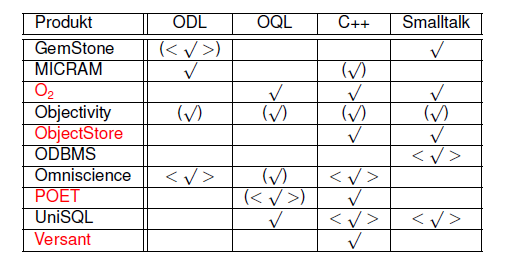
\includegraphics[scale=0.6]{img/odmg_konformitaet_1997.png}
	\end{figure}
	
	\item \textbf{Grundkonzepte}
	\begin{itemize}
		\item Objekte: Zustand direkt Bestandteil des Objektes (atomare und strukturierte Objekte); früher mutable objects
		\item Literale: Werte (atomar oder strukturiert), früher immutable objects
		\item Eigenschaften von Objekten: Attribute und Beziehungen\\
		Attribute: Werte oder Objekte\\
		Beziehungen: Objekte\\
		Beziehungen vs. objektwertige Attribute: Beziehungen immer mit inversen Referenzen, bei objektwertigen Attributen nicht
		\item Verhalten von Objekten: wird mit Operationen beschrieben (Methoden(-Schnittstellen))
		\item Typen: sammeln Objekte mit gemeinsamen Eigenschaften und gemeinsamen Verhalten\\
		\\
		\item Unterscheidung Schnittstelle und Implementierung\\
		pro Schnittstelle diverse Impl.; nicht nur bei Methoden, sondern auch im Strukturteil
		\item Typ durch Schnittstelle und mehrere Impl beschrieben
		\item Klasse ist eine konkrete Impl. dieses Typs\\
		Impl. des Strukturteils (Repräsentation der Attribute durch Datenstrukturen oder Methoden)\\
		Impl. des Verhaltensteils durch eine Menge von Methoden
		\item Def. von Schnittstellen und Impl\\
		Für Schnittstellendef. ODL oder PL-ODL\\
		Def. der Impl. sprachabhängig (C++, Java,...)\\
		\\
		\item Typhierarchie: Strukturvererbung und Vererbung von Methoden (in ODMG: Operationen; Substituierbarkeitsprinzip), Overriding
		\item Implementierungshierarchie: auf Klassen auch Impl.hierarchie (Wortsymbol extends); keine Mehrfachvererbung
		\item Instanzen: Instanz eines Typs ist (erzeugtes) Objekt von diesem Typ; virtuelle Typen (abstrakte Typen, abstract types in ODMG) haben keine Instanzen
		\item Extension: aktuelle Objektmenge einer Klasse; definierbar für jede Klasse; alle Instanzen des Typs werden Elemente der Extension
		\item tiefe Extension: Extension einer Unterklasse Teilmenge der Extension der Oberklasse (aber kein Rollenkonzept)
		\item Schlüssel: gilt für Extension der Klasse
	\end{itemize}
\end{itemize}

\subsection{Der Strukturteil und höhere Konzepte des ODMG-Standards}
\begin{itemize}
	\item Objekte haben Objektidentität und evtl Namen
	\item Lebensdauer eines Objektes zur Erzeugungszeit festgelegt
	\item \textbf{Objektidentität}\\
	Test auf Identität: Operation \textit{same\_as}\\
	Erzeugung von Objekten durch Konstruktor-Operation (vordef. Schnittstelle: factory interfaces)\\
	persistente und transiente Objekte können zu einem Typ gehören und können auch mit den gleichen Operationen manipuliert werden
	
	\item \textbf{Namen}\\
	Objektidentität nach außen nicht sichtbar\\
	falls keine Extension: benannte Objekte sind DB-Einstiegspunkte
	
	\item \textbf{Collection-wertige Objekte}
	\begin{itemize}
		\item OODM: Objekte immer unstrukturiert (atomar)
		\item ODMG: die beiden Bestandteile zusammengezogen (nicht bei tupelwertigen Zuständen: atomare Objekte mit einem tupelwertigen Zustandstyp)
		\item ODMG-Objektmodel nähert sich den OOPL-Modellen wie C++, Java an\\
		Set<T>, Bag<T>, ... T bestimmt Elementtyp der Collection
		
		\item vordef. Operationen\\
		Erzeugung: new\_of\_size (in long size)\\
		über die collection factory interfaces, initiale Größe durch size\\
		Tests: cardinality, is\_empty, contains\_element\\
		Update-Operationen: insert\_element, remove\_element\\
		Iteratoren: create\_iterator,..\\
		....
	\end{itemize}
	
	\item \textbf{Werte oder Literale}
	\begin{itemize}
		\item atomatore Typen\\
		(unsigned) long/short, float, double, bollean, char, string, enum
		
		\item komplexe Typen (collection-wertig)\\
		set<t>, bag<t>, list<t>, array<t>, dictionary<t,w>
		
		\item komplexe Typen (tupelwertig)\\
		vordef. Tupeltypen date, time, interval, timestamp\\
		Typ struct mit Operationen set\_element,..
	\end{itemize}
	
	\item \textbf{Schnittstellen}\\
	def. mit interface Klausel der ODL\\
	\textbf{Atribute}
	\begin{itemize}
		\item können mit Werten oder Methoden realisiert (gute Einkapselung)
		\item Bsp:
		\begin{lstlisting}
		interface PERSON_S
			{
		attribute long PANr;
		...	...
		attribute date Geburtsdatum;
		attribute unsigned short Alter;
		}
		\end{lstlisting}
		\item Impl. von Alter ist noch völlig frei
		\item Attribut: unidirektionale Referenz zu Komponententyp
	\end{itemize}
	\textbf{Beziehung}
	\begin{itemize}
		\item bidirektionale Referenz zu Komponententyp (Konsistenzchecks)
		\item Beispiele
		\begin{lstlisting}
		interface Student_S : Person_S {
		attribute long Matrnr;
		...	...
		attribute Person_S Mutter;
		relationship Angesteller_S Betreuer
			inverse Angesteller:S::Betreut;}
		\end{lstlisting}
		korrespondierende Klausel des Betreuers in Typ Angestellter\_S
		\begin{lstlisting}
		interface Angestellter_S : Person_S {
		attribute long Angnr;
		...	...
		relationship Set<Student_S> Betreut
			inverse Student_S::Betreuer}
		\end{lstlisting}
		
		\item ist 1:n Beziehung; 1:1 und n:m über Typen steuern
	\end{itemize}
	
	\textbf{Operationen}\\
	durch Signatur (Namen der Operation, name und Typ der Argumente und Ergebnis, Namen ovn Ausnahmen)\\
	Vererbung, Overriding (Overloading genannt), dynamisches Binden
\end{itemize}

\begin{figure}[!h]
	\centering
	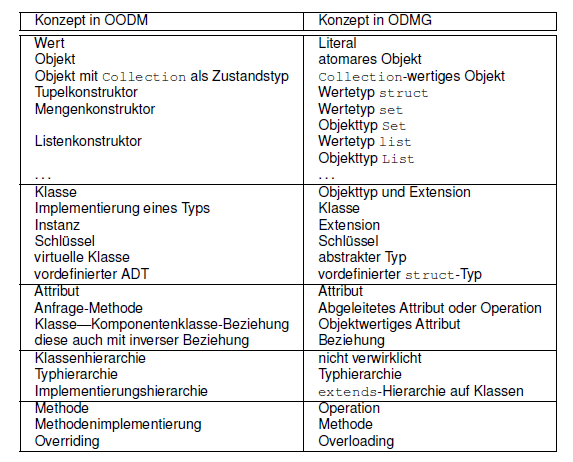
\includegraphics[scale=0.6]{img/odmg_summary.png}
	\caption{Zusammenfassung Vergleich}
\end{figure}
\newpage
\subsection{Die ODL des ODMG-Standards}
\begin{itemize}
	\item definiert Schnittstellen, Klassen 
	\begin{lstlisting}
	interface <Name> : <Obertypen>
		{<Schnitstellenspezifikation>}
	class <Name> extends <Oberklassen> : <Obertypen>
		(extent <Extension>
		keys <Schluesselmenge>)
		{<Schnittstellenspezifikation>}
	\end{lstlisting}
	
	\item Schnittstellenspezifikation
	\begin{lstlisting}
	[readonyl] attribute
		<Typ>
		<Attributname>
		
	relationship
		<Typ>|<Collection-Typ>< <Typ_1> >
		<Attribut_1>
		inverse <Typ_2>::<Attribut_2>
		
	/* fuer Operationen:
	<Typ>| void
		<Operationenname>
		(<Param_1>, ..., <Param_n>)
		raises (<Ausnahmen>)
	\end{lstlisting}
	
	\item Definition der Parameter
	\begin{lstlisting}
	on | out | inout
	<Typ><Parametername>
	\end{lstlisting}
	
	\item Typ- und Impl.hierarchie
	\begin{table}[!h]
		\centering
		\begin{tabular}{|p{10em}||p{15em}|p{15em}|}
			\hline
			&	Typhierarchie	& Implementierungshierarchie\\
			\hline
			\hline
			Obertyp	& Schnittstelle	& Klasse\\
			\hline
			Untertyp	& Schnittstelle oder Klasse	& Klasse\\
			\hline
			Art der Vererbung	& Mehrfachvererbung	& Einfachvererbung\\
			\hline
		\end{tabular}
	\end{table}
	\item Klassenhierarchie ermöglicht keine Mehrfachvererbung
\end{itemize}

\subsection{Der Operationenteil und die OQL des ODMG-Standards}
\begin{itemize}
	\item Object-Query-Language ist Anfragesprache basierend auf SFW-Block von SQL-92
	\item zusätzlich: komplexe Werte, Objektidentitäten, Pfadausdrücke über Komponentenobjekte hinweg, Methoden, Overriding von Methoden\\
	nicht nur Mengen, sondern allgemeien Collection\\
	neben dem SFW-Block auch bel. andere Anfrageblöcke
	\item funktionale, orthogonale Sprache
	\item Grundprinzip einer Anfrage: Ausgangspunkt -> Name eines atomaren, strukturierten oder Collection-wertigen Objektes oder Wertes\\
	Name der Extension des Typs Person
	\begin{lstlisting}
	Personen
	\end{lstlisting}
	ist gültige Anfrage (Collection-wertiges Objekt)
	\item \textbf{SFW-Block} wird zum Filtern von Mengen eingesetzt wie bei
	\begin{lstlisting}
	select distinct struct (f: s.Studienfach, b: s.Betreuer)
	from Studenten s
	where s.Adresse.Ort = 'Rostock'
	\end{lstlisting}
	In dieser Anfrage wird die Extension Studenten nach dem Wohnort 'Rostock' gefiltert.\\
	Adresse kein Attribut des Typs Student, aber vom Obertyp Person vererbt\\
	Ort Komponenten des Strukturierten Attributs Adresse, mit Pfadausdruck erreichbar
	
	\item Relationale und objekterzeugende Anfragen
	\begin{itemize}
		\item relationale Anfrage: letzte Anfrage nach Rostocker Studenten
		\item objekterzeugende Anfrage: statt des Typkonstruktors struct Objektkonstruktor (In ODL def. Typen)
		\begin{lstlisting}
		Person (PANr: 8883494,
			Name: struct (Vorname: 'Otto', Nachname: 'Ohnmacht'),...)
		\end{lstlisting}
		erzeugt neues Objekt vom Typ Person\\
		Objekte hier jedoch nur für bestehende Typen\\
		keine dynamische Typisierung und Klassifizierung
	\end{itemize}
	
	\item Objekterhaltende Anfragen
	\begin{itemize}
		\item Objektidentitäten der Rostocker Studenten in einer Multimenge aufsammeln
		\begin{lstlisting}
		select s
		from Studenten s
		where s.Adresse.Ort = 'Rostock'
		\end{lstlisting}
		
		\item keine dynamische Klassifizierung oder Typisierung des Anfrageergebnisses
		\item extensionsbasierte, keine klassenbasierte Anfrage
		\item Rostocker Studenten bilden neue Extension vom Typ Student als Anfrageergebnis, jedoch keine dynamisch erzeugte Unterklasse von Student
		\item auch Typ der Objekte nicht veränderbar
	\end{itemize}
	
	\item \textbf{Orthogonalität}
	\begin{itemize}
		\item auf jede Collection Anfrageioerationen anwendbar
		\begin{lstlisting}
		select z.Fach
		from Huho.Zeugnis z
		\end{lstlisting}
		liefert eine Multimenge von STRINGs, die Prüfungsfächer des Studenten Hugo
		\item Menge von Prüfungsfächern aller Studenten
		\begin{lstlisting}
		select distinct z.fach
		from Studenten s, s.Zeugnis z
		\end{lstlisting}
	\end{itemize}
	
	\item \textbf{Nullwerte}
	\begin{itemize}
		\item Gewöhnungsbedürftig: Behandlung von undef. Objekten 
		\item Laufzeitfehler bei 
		\begin{lstlisting}
		select s.Betreuer
		from Studenten s
		\end{lstlisting}
		falls Betreuer mindestens eines Studenten nicht def.
		\item korrekte oder 'sichere' Anfrage wäre gewesen
		\begin{lstlisting}
		select s.Betreuer
		from Studenten s
		where is_defined (s.Betreuer)
		\end{lstlisting}
	\end{itemize}
	
	\item \textbf{Ausnutzung von Typkonstruktoren und Klassenhierarchie}
	\begin{itemize}
		\item OQL erlaube direkt Vergleich von Mengen
		\begin{lstlisting}
		select b
		from b in Buecher
		where set(RDBS, lehrbuch) >= b.Stichworte
		\end{lstlisting}
		OQL bietet Mengenoperationen an, aber folgende nicht erlaubt
		\begin{lstlisting}
		Ausleihobjekte union Geraete
		\end{lstlisting}
		nur Mengen mit gleichen oder vergleichbaren Elementtypen können vereinigt werden (alle in Anfragen auftretenden Klassen müssen def. sein, Typ des Ergebnisses muss eindeutig sein)
		\item Unvergleichbare Klassen können mehr als eine kleinste gemeinsame Oberklasse haben: Eindeutigkeit nicht gegeben
		\item haben sie überhaupt keine gemeinsame Oberklasse, ist das Ergebnis nicht einmal darstellbar
	\end{itemize}
	
	\item Pfadausdrücke einmal anders: geschachtelte Anfrage; relationale Anfrage
	
	\item weitere Klauseln
	\begin{itemize}
		\item Quantoren for all und exists
		\item Sortierung sort und Gruppierung group by mit having
		\item Aggregatfunktionen im Umfang von SQL
		\item Def. temporärer Relationen mit defined
		\item Operationen zur Typkonvertierung wie listtiset und flatten
		\item Aufruf bel. Methoden in jeder Klausel
		\item völlige Orhtogonalität
		\begin{lstlisting}
		max(select Gehalt from Angestellte)
		\end{lstlisting}
		im Gegensatz zu Standard-SQL erlaubt
	\end{itemize}
\end{itemize}

\subsection{Umsetzung in OODBPL-Systemen}
\begin{itemize}
	\item OODBPL: üblicherweise auf ODMG basierend
	\item einige Umsetzungen:\\
	O$_2$: ODMG-OQL\\
	Ontos: eigenes Object SQL...
	
	\item ODMG Sprachanbindung
	\begin{itemize}
		\item einheitliches Typsystem zw Programmiersprache und DB:\\
		Die für die ODL-Konzepte erzeugten PL-Klassen mit ihren Methoden können persistente oder transiente Objekte aufnehmen; ODL-Klassen bilden Teil der PL-Klassenbibliothek.
		\item Einbettung erfolgt in Syntax der Programmiersprache; soll den ''impedance mismatch'' relationaler Embedded-SQL-Versionen vermeiden
		\item Ergänzungen der Klassenbibliotheken so klein wie mgl halten; Methoden fü deskriptive Anfragen und Transaktionsverwaltung hinzufügen
		\item BD- und OOPL-Teile frei kombinierbar
		\item persistente und transiente Objekte können zu einer Klasse gehören
	\end{itemize}
	
	\item Fazit: ODMG Einschränkungen\label{odmg_constraints}
	\begin{itemize}
		\item Objekt fixiert in einer einzigen Klasse (keine Mehrfachzugehörigkeit, kein Klassenwechsel)
		\item kein orthogonales Typkonzept
		\item Programmiersprachensemantik statt Datenbanksemantik
		\item nur extensionsbasierte Anfragen, keine klassenbasierten Anfragen
		\item Mehrfachvererbung: nur Interfaces, keine Implementierung
		\item Persistenzprinzip: jedes Binding reagiert anders
	\end{itemize}
	
	\item Planung in ODMG nicht behandelt -> siehe VL Folien (halte ich nicht für prüfungsrelevant)
	\item ODMG Stand 2015
	\begin{itemize}
		\item seit 2006 geplant, 2014 eingestellt
		\item JDO als einzige Sprachanbindung von Java zu OODBMS
		\item seit 2006 JPA als Sprachanbindung von Java zu RDBMS 
	\end{itemize}
\end{itemize}